In this chapter, we talk about state-of-the-art technologies in computer vision and how we have used them for remote sensing problems. We also give a brief account of natural disaster assessment, and how are these machine techniques applied in this sense. We use the Chiapas earthquake that happened on September 7, 2017, as a study case because of the data that was publicly made available by the CENAPRED.\\

An excellent introduction to neural networks in the context of remote sensing is in \cite{canty2014image}. It reviews all the necessary mathematical tooling to deal with the processing image algorithms and implements them in an interpreted high leve language called Python. A survey of distinct aspects of how to transfer learning from separate domains is in \cite{5288526}.\\

\section{Damage Assesment}

In the field of natural disasters, we found many references to work that takes advantage of datasets in many different forms. For example Kryvasheyeu \textit{et al.}, in 2016, used the twitter activity during  Hurricane Sandy to build a model. They found that social media activity correlates with the proximity of the region in which the Hurricane hits \cite{Kryvasheyeue1500779}. Nevertheless, they mention that the nature of the data available both in quantity and quality is unusual in part because of the severity and magnitude of damage that the Hurricane Sandy brought about.\\

A close approach to what we propose is the work of Rashedi and Mori \cite{Nia2017BuildingDA}. They gathered a dataset of damaged building images from different sources and gave them a numerical degree of damage. They used these data to train a model consisting of three different pipelines that extracted features of diverse natures, and then used this features to obtain a single continuous value using a sigmoid function. This technique is useful in the sense that it does not require to have images of the state of the building previous to the disaster.\\


\section{Convolutional Neural Networks}

We found ongoing research about the idea of using features crafted by a neural network in different domains. We took inspiration from some of these techniques for our research framework. This field is still novel and will be expanding in future years.\\

Jeff Donahue \textit{et al.} developed a framework which they called Deep Convolutional Activation Features (DeCAF) \cite{DBLP:journals/corr/DonahueJVHZTD13}. They feed traditional methods with the features extracted from the CNN obtaining accuracies compared to state of the art methods at the time. They took the activations from the $n^{th}$ hidden layer, the layer previous to the one that is fully connected, and use them to train two classifiers: a logistic regression, and a support vector machine, in four different environments: object recognition, domain adaptation, subcategory recognition and scene recognition. Object recognition tested the ability of the classifier to assign a class to a given image correctly. They showed that the depth of the layer dramatically improves the performance of the features. Domain adaptation consists of testing the robustness of the classifier when the source of the image varies, in this case, they use a testing-set consisting of images of office objects taken from Amazon, a webcam, and a DSLR camera. The classifiers were able to cluster the objects across domains regardless of the origin of the images. In subcategory recognition, the task at hand is to differentiate individual categories inside a super-category, for example, discriminate among two types of birds using a training set consisting only of images of birds. They found that without further fine-tuning, the features extracted from the neural network achieved accuracies far superior to the ones available in the literature at the time. Finally, they tested the extracted features at the task of semantical classification. Instead of requiring the classifier to give a category for the object in the picture, the classifier must semantically classify the scene instead. The task above is considered extremely difficult, and the previous approach was to use hand-engineered features and a multi-kernel learning baseline. While the accuracies reported by this task were quite low, they improved the existing benchmark which provides strong evidence that the features extracted from the deeper layers of a CNN excel at extracting information from the images even though the original design of the network was different. Additionally, they developed an open source framework that later matured into Caffe \cite{jia2014caffe}, a framework designed to train CNN models.\\

Another attempt that adds to the evidence that features engineered by the Neural Network work pretty good off the shelf, is Razavian \texttt{et al.} \cite{DBLP:journals/corr/RazavianASC14}. They use features extracted from the CNN \texttt{OverFeat} model which was made public by Le Cun \textit{et al.} \cite{DBLP:journals/corr/SermanetEZMFL13}. In the original article, they explore the advantages of training a network simultaneously for several tasks in this case: classify, locate and detect objects in images. Razavian \texttt{et al.} experiment with these features to perform classification in tasks that gradually move away from the one for what \texttt{OverFeat} excel. They tested the features extracted from the CNN model together with a traditional support vector machine in the tasks of image classification, fine-grained recognition, attribute detection, and visual instance retrieval. They found that the CNN proved to be a strong competitor against more sophisticated methods involving handmade features.\\

Transfer learning consists of using the knowledge acquired by a model during a training phase to another domain of knowledge. It is explored by Yosinski \textit{et al.} in \cite{DBLP:journals/corr/YosinskiCBL14}. They propose to use an already trained architecture in new tasks by replacing different layers and retraining only the topmost layers. An experiment was designed to test the transferability of different layers. They found strong evidence that suggests that even though the training sets are of different nature, features transferred from different tasks improve the performance of the CNN against random weights. They used ImageNet \cite{Deng09imagenet:a} splitting the dataset obtaining two different groups of images. They also found that the transferability is negatively affected by the deepness of the layers, meaning that higher layer features are specialized to the given task. This idea gave us a clear starting point for the task in our hands.\\

\begin{figure}[!h]
  \centering
    \begin{subfigure}{.8\textwidth}
        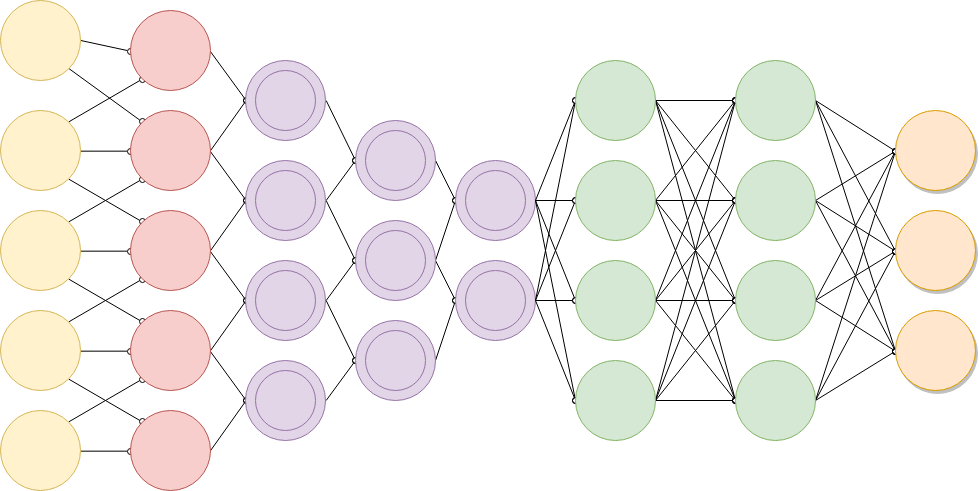
\includegraphics[width=\textwidth]{images/transfer2.png}
        \caption{Task A}
    \end{subfigure}
    \begin{subfigure}{.8\textwidth}
        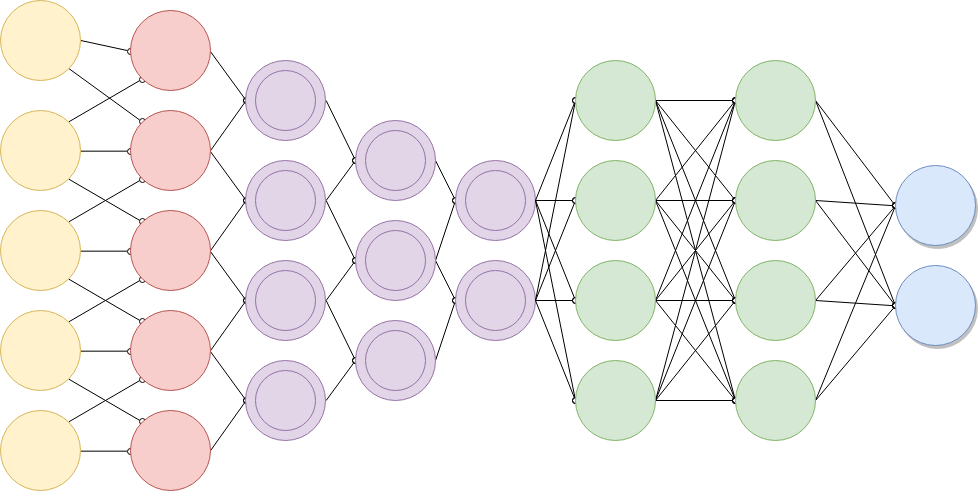
\includegraphics[width=\textwidth]{images/transfer1.png}
        \caption{Task B}
    \end{subfigure}
  \caption{A graphical representation of how transfer learning works. The last layer of the architecture is changed while leaving the rest without modification.}
  \label{fig:juchitan}
\end{figure}


Image segmentation is another task that has been explored using neural networks. The idea is to obtain a semantic partition of the images. In our case, it would be desirable to have a heat map that can separate the damaged buildings from the rest of the elements of the image. In \cite{DBLP:journals/corr/LongSD14} Long \textit{et al.} use the features extracted from the CNN to segment such an image. They modified the architecture of several classification networks into fully convolutional networks, and the features learned were fine-tuned for the segmentation task. This process is very promising for the field of Remote Sensing where we engineer classification features by using traditional methods such as manipulating the image information without taking into account the semantic context. Other fields, such as biomedicine, also explored this topic \cite{DBLP:journals/corr/RonnebergerFB15}.\\

The possibility of having a single model that can perform well in many different tasks is explored in \cite{DBLP:journals/corr/KaiserGSVPJU17}. Kaiser \textit{et al.} aimed to create a single model capable of performing well in very different tasks. They noticed that while CNNs give impressive results in a variety of functions, they need to repeat training efforts for every situation. They created an architecture capable of receiving training data from 8 different corpora, ranging from image classification to language translation or natural language processing. Given the very different nature of the training data, they needed to create encoders to transform it into a joint representation space. Several tasks such as translation from English to German and translation from French to English shared the same encoders promoting stronger generalization of the features. Finally, they found that the domains in which the data is limited are benefited with the joint training while the other tasks suffer from little or no loss of accuracy at all. While not achieving state of the art results in any of the domains, they found that it is indeed possible to train a model to learn many different objectives. \\


Zhou and Prasad used an idea known as active learning to improve the performance of a classifier taking the most of small labeled datasets \cite{7956153}. Active learning is based on the observation that the traditional approach of randomly selecting training samples leads to redundancy in the training sets. The approach is to enable the learner to select the most informative training data. In their research, they explore the use of active learning together with semi-supervised learning techniques.\\

\section{Computer Vision}

Neural networks appeared as function approximators that could be adjusted to simulate the behavior of linear functions. As they grew in sophistication, new architectures were capable of performing well in more complex tasks. The pioneer in using them for image recognition was Yann LeCun in 1990.\\

Le Cun \textit{et al.} \cite{119325} proposed to use an architecture of a multilayer neural network that was able to learn directly from the data with no prior feature extraction. Instead of using a fully connected network, they proposed a locally connected net. It was capable of extracting local features and passed them down to the subsequent layers in what they called a \textit{feature map}. Each unit took the information of a $5\times 5$ neighborhood of the pixel in the previous layer. The last layer of the architecture consisted of ten classes that represented each of the possible digits. This design, which was trained using backpropagation, is what now we know as CNNs. The reason that their research was so groundbreaking was that their architecture needed very little information about the task it was performing. They were able to extend the use of their method to other symbols; however, they state that the technique was not able to be applied to very complex objects. With the tremendous advances that computer power has suffered in the late years, this has been proven to be incorrect. In 2009 a prominent image database was gathered and published \cite{Deng09imagenet:a}. Ever since this happened, this database became the defacto dataset to test classification methods. A few years later, in 2012 Krizhevsky \textit{et al.} \cite{krizhevsky} proposed the use of CNNs in the daunting task of classifying the image dataset.\\

The use of neural networks to automatically detect roads was explored already before CNNs became widely used in computer vision tasks \cite{Mnih:2010:LDR:1888212.1888230}. They proposed a simple architecture with a single hidden layer. They use the now standard procedure of cropping small patches from the complete image and worked on the RGB color space. They used aerial imagery in addition to vector information on roads as training data. Instead of manually tagging the photos they proposed a model that assumes a certain amount of thickness in the streets, which usually have no dimension. To reduce the input dimensionality, they applied Principal Component Analysis (PCA), keeping the most informative principal components. As a method of post-processing, they use a neural network to reduce the noise in the images, efficiently getting rid of false positives and false negatives by using context information. One of the valuable lessons learned from this experiment is the value of the random rotations in the training data. It is common that road networks in cities create grids, they realized that a model trained with information from a particular town would perform poorly if data from a new one is shown to the model, to put it in another way, the model generalized poorly. They found that we can relive this if we applied random orientations to the data as when we are dealing with bird-eye sight, and there is no correct orientation for images. They also found that pre-processing the pictures with methods such as edge detection showed no improvement in the performance of their pipeline, they attributed this to the fact that the neural network crafts features of this nature when learning to perform the task of recognizing roads.\\

Another attempt to use features extracted from a CNN in a different context is in Michael Xie \textit{et al.} \cite{DBLP:journals/corr/XieJBLE15}. They examine this approach by training a CNN on top of the well-known \texttt{VGG F} model. First, they replace the fully connected layers on top of that model with a convolutional layer. Then they re-train the features the model learned from ImageNet with aerial images and nighttime images gather from the National Oceanic and Atmospheric Administration (NOAA). While they get excellent accuracy results from using daytime images to predict nighttime light, it was not the purpose of their research. Instead, features crafted by the network are extracted and used to train a model to predict poverty from satellite imagery. To do so, they use these features as input for a logistic regression classifier. To compare their model, they train four other models extracting features from a survey, features from ImageNet itself, features from the nighttime light intensities and features from ImageNet and nighttime light strengths at the same time. The transfer model outperforms every model except for the one based on survey data, which strongly suggests that the transfer learning technique is extracting complex information from the aerial scenes. They clarify that although this approach can be useful when conducting surveys is prohibitively expensive.\\

\section{Remote Sensing}

In recent years groundbreaking advances in computer vision have led to tremendous advances in other science fields. These algorithms are behind many of the tools that we use every day, and that we take for granted. Nowadays face recognition techniques are so advanced that we can use them as an authentication method. Autonomous vehicles are soon to be a reality, reshaping the way we move. We can build three-dimensional models from hundreds of overlapping images \cite{Szeliski:2010:CVA:1941882}. In particular, we are interested in the field of remote sensing.\\

Remote sensing is a field that studies the energy emanating from the earth's surface and captured by a sensor mounted in an aerial vehicle or a satellite \cite{richards2013remote}. Landcover classification is one of the most important disciplines in the field. In the case of digital imagery, we want to classify pixels into clusters of interest to extract information from the raw data that the sensors acquire. In our case, we want to detect pixels that represent damaged buildings automatically.\\

Kussul \textit{et al.} \cite{7891032} explored the use of CNNs in the context of land-cover classification. They used an ensemble of CNNs to obtain state of the art results in the classification of different types of crops using multitemporal and multisensor satellite data. They explore two approaches. First, they use a 1-D CNN to perform the convolutions in the spectral domain by stacking the different bands from the Sentinel-1 A and Landsat-8 sensors. This process outputs a pixel-wise classification; they then use a traditional 2-D CNN on the images. To not lose resolution with the 2-D CNN, they use a sliding window approach assigning the class to the center pixel of the sliding window. Finally, they ensemble both opinions and filter the result to improve the quality of the map.\\

The usual approach with landcover classification is the use of classical classification methods such as support vector machines (SVM) and random forests (RF). To improve the performance, we must handcraft features from the original bands. In \cite{7858676}, Grant \textit{et al.} explore the use of the mentioned above method of transfer learning and data augmentation in the context of remote sensing images. They tested their methods with well-known high-resolution datasets, and they obtained state of the art results.\\

In \cite{DBLP:journals/corr/KendallBC15} and \cite{DBLP:journals/corr/BadrinarayananK15}, Kendall \textit{et al.} propose and enhance their own approach by extending their architecture to include a Bayesian approach. The idea is to add a model of uncertainty to the CNN and use this information to get more accurate guesses on each of the pixels. They report that this feature adds some improvement in the level of accuracy for many types of architectures not only their SegNet.\\

\section{Data Augmentation}

Data augmentation is a technique used to artificially increment the size of the training dataset by applying an affine transformation to the images. When tagged data is scarce and difficult to obtain this method is a good choice. Frequent alterations that the photos are subjected to include rotations and reflections. When we choose to use this technique we should be careful about the orientation of the objects, for example, a building upside down makes no sense, so there is no use to create the network learn features on objects that it will not see in a real situation. Fortunately, aerial imagery does not present this problem. No particular orientation is considered correct with aerial pictures. This case means that we can dramatically boost the size of our dataset without the cumbersome process of manually tagging.\\

The reasoning behind this idea is that when we see a picture, our brain automatically orients it into its correct position. Showing the network an image with different positions and orientations of an object we enrich its knowledge about it, we can see an example in Figure \ref{fig:rotate}.\\

\begin{figure}[!h]
  \centering
    \begin{subfigure}{.24\textwidth}
        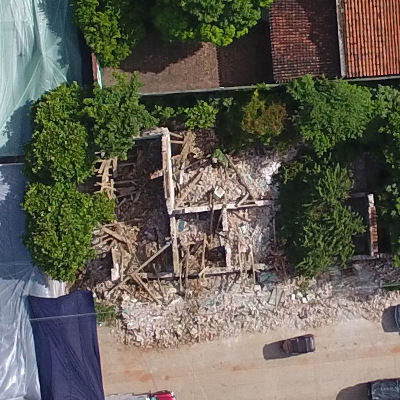
\includegraphics[width=\textwidth]{images/rotation4.jpg}
    \end{subfigure}
    \begin{subfigure}{.24\textwidth}
        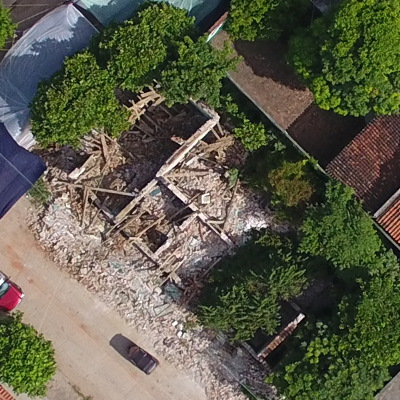
\includegraphics[width=\textwidth]{images/rotation3.jpg}
    \end{subfigure}
    \begin{subfigure}{.24\textwidth}
        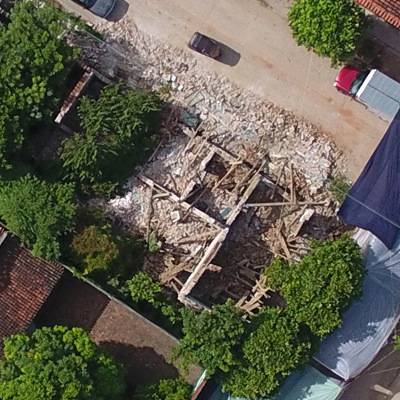
\includegraphics[width=\textwidth]{images/rotation1.jpg}
    \end{subfigure}
    \begin{subfigure}{.24\textwidth}
        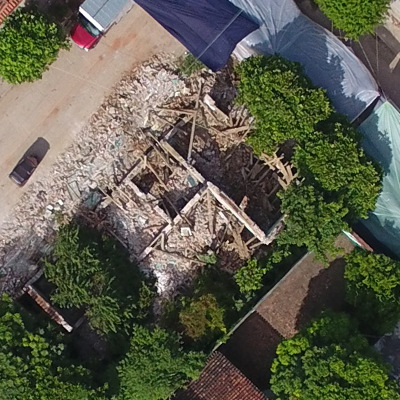
\includegraphics[width=\textwidth]{images/rotation2.jpg}
    \end{subfigure}
  \caption{Same image with different rotations. A way to boost the size of the training set.}
  \label{fig:rotate}
\end{figure}

\section{TensorFlow}

TensorFlow is a machine learning system developed by the Google Brain Team to supersede its first-generation system, DistBelief. Built on top of the lessons learned during DistBelief development. One of the fundamental concepts that lead the team to create a new system from scratch was the need for flexibility. TensorFlow lets us express machine learning algorithms using a standard interface with implementations targeting a wide range of devices. Complex models that first implemented in DistBelief such as Inception got a performance boost of a factor of x6 \cite{tensorflow2015-whitepaper} when they got moved to the new system. TensorFlow was opened sourced on November 9, 2015 under the Apache 2.0 license.\\ 

In this section, we will untangle some of the details of how TensorFlow and its graph model work \cite{DBLP:journals/corr/AbadiBCCDDDGIIK16}. It uses an elegant data-flow system in which both the operations and the state of the algorithm get represented as nodes and edges in a directed graph. This lets the system build an optimal sub-graph before starting the calculations.\\

With flexibility in mind, this system lets the user define new operations and register them to use within the framework. Additionally, it was developed to target different platforms, from machine clusters to mobile devices, these implementations are known as \textit{kernels}. Using the same programming model, TensorFlow decides at runtime which pieces to use; this is useful when taking into account the whole development process of a data product and how it evolves. For example, when a developer experiments with data in a single computer before deploying the system to be trained with a more massive data set in a cluster of computers. Another example comes when the model training process, it can be deployed to an online service which will run on a single computer, but then it can be implemented in a mobile device for offline use. In each of these steps the underlying environment is entirely different. However, TensorFlow adapts automatically to each situation.\\


As a standard interchange data format, it uses tensors. With machine learning algorithms, it is often the case to have sparse data, encoding it as dense tensors is a smart way to save space. As we mentioned before, TensorFlow uses a graph to represent both the state and the operations. Nodes represent operations. Edges represent inputs and outputs between these operations. The system takes its name from the tensors flowing through this pipes. Although it is not of particular importance to our experiment, it is worth mentioning that TensorFlow supports algorithms with conditional and iterative control flow, which means that we can use it, without further tuning, to train Recurrent Neural Networks which are very important in fields like speech recognition and language modeling.\\

The system also provides a library that allows symbolic differentiation. As many machine learning techniques rely on Stochastic Gradient Descent to train a set of parameters, this feature makes more comfortable to explore new techniques as the framework produces backpropagation code for any combination of operation nodes.\\

They built TensorFlow with considerably large data-sets in mind. It provides an intern library that allows the distribution of datasets that would be too large to fit in RAM. Instead, data can be sliced, taking advantage of how some algorithms work. Additionally, communication between nodes uses lossy compression, taking advantage of the fact that some of the machine learning algorithms are tolerant to reduced precision arithmetic. It is important to mention that it is possible to extract state and information from any particular node in the graph. This fact is fundamental to our study because we are interested in the features that the system craft to perform the given task. We want to teach the system to excel at our task of interest and then use its knowledge to improve another task.\\

Another feature that TensorFlow provides is its ability to prune the execution graph before starting its computations. Usually, several sets operations repeat along the graph, by detecting this, the system can automatically replace all incidences of each repeated sub-graph with a single one thus, saving memory and time. The same case happens with communication nodes. If several nodes from a single device are consuming the same data from another device, the system is prepared to detect this and ensure that the data transfer occurs only once.\\

The framework code is deeply optimized. They built it upon known mature frameworks such as cuDNN, a library for deep neural networks that targets NVIDIA GPUs, and Eigen, a C++ library for linear algebra, which was extended to offer tensor arithmetic support. On top of this infrastructure, TensorFlow offers a Python client which is very convenient for fast development.\\

An interesting tool that comes with the framework is TensorBoard. With the immense complexity that machine learning models offer at this scale, it is essential to know what is happening at any point in the training process. TensorBoard offers a glimpse of how the architecture for a particular computation graph looks. This tool will become handy later when describing our model.\\

There are several alternatives that offer similar features to TensorFlow. Theano, Torch, Caffe, Keras to name a few. The purpose of this work is by no means to study the advantages or disadvantages of these systems nor to create a benchmark for their performance. We choose TensorFlow because the pipeline was already in Python,  to minimize the gluing code. Among the examples that come with the system, there is an end to end example of how to transfer learning from one trained net to another task.\\

\section{Summary}

An extensive literature review gave us the tools to plan our methodology, based on the ideas that we thought were promising for our objective. Given the results reported in \cite{DBLP:journals/corr/YosinskiCBL14}, we decided to use transfer learning for our task. We decided not to explore the concept of data augmentation because we had the ability to control the size of the training set. We took the tool that TensorFlow provides to perform transfer learning, using Inception as the architecture to start with. Based on \cite{DBLP:journals/corr/RazavianASC14}, we choose to compare the method using transfer learning with a more classical approach, in our case we chose a random forest classifier. To keep the scope of our work not too ambitious we left out the possibility of collating our results with official data as suggested on \cite{Kryvasheyeue1500779}.






